\documentclass[12pt]{article}

\usepackage{amssymb,amsmath,amsthm,chngcntr,makeidx,fancyhdr,rotating,graphicx,hyperref,mathtools}

\usepackage[a4paper,bottom=3cm,hmargin={2cm,2cm}]{geometry}
%\usepackage[dutch]{babel}
\usepackage[all]{xy}
\usepackage[T1]{fontenc}
%\usepackage{pstricks-add}
\usepackage{booktabs}
\usepackage[demo]{graphicx}
\usepackage{caption}
\usepackage{subcaption}
\usepackage[shortlabels]{enumitem}

\usepackage{svg}

\usepackage[]{tikz}
\usetikzlibrary{intersections,positioning,calc,arrows}
\usepackage{pgf,pgfplots}
\pgfplotsset{compat=1.15}
\usepackage{mathrsfs}
\usepackage{xparse}
\usetikzlibrary{calc,angles,positioning,intersections,quotes,decorations.markings}

\mathtoolsset{centercolon}

\makeatletter
%\newcommand{\xleftrightarrow}[2][]{\ext@arrow 3359\leftrightarrowfill@{#1}{#2}}
\newcommand{\xdashrightarrow}[2][]{\ext@arrow 0359\rightarrowfill@@{#1}{#2}}
\newcommand{\xdashleftarrow}[2][]{\ext@arrow 3095\leftarrowfill@@{#1}{#2}}
\newcommand{\xdashleftrightarrow}[2][]{\ext@arrow 3359\leftrightarrowfill@@{#1}{#2}}
\def\rightarrowfill@@{\arrowfill@@\relax\relbar\rightarrow}
\def\leftarrowfill@@{\arrowfill@@\leftarrow\relbar\relax}
\def\leftrightarrowfill@@{\arrowfill@@\leftarrow\relbar\rightarrow}
\def\arrowfill@@#1#2#3#4{%
  $\m@th\thickmuskip0mu\medmuskip\thickmuskip\thinmuskip\thickmuskip
   \relax#4#1
   \xleaders\hbox{$#4#2$}\hfill
   #3$%
}
\makeatother

\theoremstyle{plain}
\newtheorem{theorem}[subsection]{Theorem}
\newtheorem{corollary}[subsection]{Corollary}
\newtheorem{proposition}[subsection]{Proposition}
\newtheorem{lemma}[subsection]{Lemma}
\theoremstyle{definition}
\newtheorem{definition}[subsection]{Definition}
\newtheorem{example}[subsection]{Example}


\renewcommand{\baselinestretch}{1.2}
\setcounter{MaxMatrixCols}{20}

\let\epsilon=\varepsilon
\let\phi=\varphi
\let\simeq=\cong


\newcommand{\se}[1]{\begin{equation*}
    \begin{split}
        #1
    \end{split}
\end{equation*}}
\newcommand{\sm}[1]{\left(\begin{smallmatrix}
        #1
\end{smallmatrix}\right)}

\newcommand{\Isom}{\mathsf{Isom}\,}
\newcommand{\A}{\mathbb{A}}
\newcommand{\B}{\mathbb{B}}
\newcommand{\C}{\mathbb{C}}
\newcommand{\D}{\mathbb{D}}
\newcommand{\E}{\mathbb{E}}
\newcommand{\F}{\mathbb{F}}
\newcommand{\G}{\mathbb{G}}
\renewcommand{\H}{\mathbb{H}}
\newcommand{\I}{\mathbb{I}}
\newcommand{\J}{\mathbb{J}}
\newcommand{\K}{\mathbb{K}}
\renewcommand{\L}{\mathbb{L}}
\newcommand{\M}{\mathbb{M}}
\newcommand{\N}{\mathbb{N}}
\renewcommand{\O}{\mathbb{O}}
\renewcommand{\P}{\mathbb{P}}
\newcommand{\RP}{\mathbb{RP}}
\newcommand{\PP}{\mathbb{P}}
\newcommand{\EE}{\mathbb{E}}
\newcommand{\Q}{\mathbb{Q}}
\newcommand{\R}{\mathbb{R}}
\newcommand{\T}{\mathbb{T}}
\newcommand{\U}{\mathbb{U}}
\newcommand{\V}{\mathbb{V}}
\newcommand{\W}{\mathbb{W}}
\newcommand{\X}{\mathbb{X}}
\newcommand{\Y}{\mathbb{Y}}
\newcommand{\Z}{\mathbb{Z}}


\newcommand{\ab}{\mathrm{ab}}
\newcommand{\Aff}{\mathrm{Aff}}
\newcommand{\Aut}{\mathrm{Aut}}
\newcommand{\Syl}{\mathrm{Syl}}

\newcommand{\diag}{\mathrm{diag}}
\newcommand{\End}{\mathrm{End}}
\newcommand{\Hom}{\mathrm{Hom}}
\newcommand{\ggd}{\mathrm{ggd}}
\newcommand{\GL}{\mathrm{GL}}
\newcommand{\gr}{\mathrm{gr}}
\newcommand{\id}{\mathrm{id}}
\renewcommand{\Im}{\mathrm{Im}}
\newcommand{\inh}{\mathrm{inh}}
\newcommand{\Image}{\mathrm{Im}}
\newcommand{\Index}{\mathrm{index}}
\newcommand{\Iso}{\mathrm{E}}
\newcommand{\kar}{\mathrm{char}}
\newcommand{\Ker}{\mathrm{Ker}}\let\ker=\Ker
\newcommand{\kgv}{\mathrm{kgv}}
\newcommand{\OO}{\mathrm{O}}
\newcommand{\ord}{\mathrm{ord}}
\newcommand{\orde}{\mathrm{orde}}
\renewcommand{\Re}{\mathrm{Re}}
\newcommand{\SL}{\mathrm{SL}}
\newcommand{\totgr}{\mathrm{totgr}}

\newcommand{\rectangle}{{\sqsubset\!\!\sqsupset}}

\definecolor{light-gray}{gray}{0.5}

\newcommand{\antwoord}[2]{{\color{light-gray}~\newline\boxed{\parbox[t][]{.99\linewidth}{{\tiny \sf ANSWER \thechapter.\arabic{question}}\\ #1}}\vspace{.2cm}}}


\newcommand{\tikzprent}[2]{\begin{center}\begin{tikzpicture}#1\end{tikzpicture}\\{\it #2}\end{center}}

\newcommand{\<}{\langle}
\renewcommand{\>}{\rangle}

\newcommand{\angstrom}{\textup{\AA}}

\usepackage[
backend=biber,
style=nature,
sorting=ynt
]{biblatex}

\addbibresource{library.bib}

\graphicspath{ {./img/} }

\author{
	Broerse, Mart\\
	\and
	Jaspers, Boris\\
	\and
	Marshall, Max
}

\title{%
  Optimization of the Figure of Merit for High Temperature Applications by Manipulation of Point Defects \\
  \large Workshop Physics and Astronomy \\ Institute for Theoretical Physics Amsterdam}
  
\date{January 2023}

\begin{document}

\maketitle

\begin{abstract}
TODO
\end{abstract}

\section{Introduction}

Thermoelectrics have the potential to play a key role in addressing one of this generation's defining crises, namely the increasing demand for sustainable energy \cite{Wang2021}. These materials can be utilised to directly convert waste heat into electrical energy, which could significantly improve the energy efficiency of processes that generate excess heat \cite{Wang2021}.
The applications of thermoelectric materials are not limited to bulk waste heat recovery, they can also be applied in devices that require precise or localised temperature control \cite{1616249}.
Thermoelectrics are solid state materials, and as a result need less maintenance and space than mechanical electric generators \cite{SnyderGJeffrey2008Ctm}.
Another benefit is that they do not produce noise, and forgo no mechanical wear \cite{SnyderGJeffrey2008Ctm}.

Examples of current thermoelectric energy generation (TEG) applications include, but are not limited to, TEG appliances designed for areas with a shortage of electricity, waste heat recovery from vehicles and cargo vessels [REF], power supplies for wireless sensors and wearable devices \cite{10.4108/icst.bodynets.2014.257119}, and the radioisotope TEG adopted in spacecrafts by NASA \cite{doi:10.2514/6.2005-5713}.  
The relatively niche market for TEG is mainly ascribed to the low TE energy conversion efficiency, high cost of TE materials, and slow progress of reliable module development [REF].

One of the main drawbacks of thermoelectric materials is their low energy conversion efficiency \cite{SnyderGJeffrey2008Ctm}; this makes them less desirable as a solution to the increasing demand for clean energy.
Other problems for the large-scale application of thermoelectrics include the toxicity of the materials \cite{LiuWei2017Ehst}, and the scarcity of the elements the materials are synthesised from \cite{LiuWei2017Ehst}, which consequently affects their cost.

Some known well-performing thermoelectric materials include V2VI3 compounds and their derivatives, where $\text{V} \in \{\text{Sb}, \text{Bi}\}$ and $\text{VI} \in \{\text{S}, \text{Se}, \text{Te}\}$, which have been used for 60 years and at multiple times have been considered mature \cite{https://doi.org/10.1002/advs.201600004}. More recently, $\text{MoSi}_{2}\text{N}_{4}$ has been used to construct a monolayer with potential for applications in catalysis and nanoelectronics \cite{MA2022153214}.

Molybdenum silicides may be suitable candidates. They are relatively non-toxic for humans \cite{NOVOTNY2018272} and while molybdenum is not an abundant element \cite{HENCKENS201861}, molybdenum silicides may be viable for industrial applications \cite{STOLOFF20001313}.
They have the added benefit of being corrosion resistant [REF], and they have a high melting point relative to other thermoelectric materials [REF], which positively affects the range of temperatures at which the material is stable.
Depending on the thermoelectric properties, this may result in a greater range at which the thermoelectric material is able to generate significant electrical energy [REF].

The key measure of the quality of a thermoelectric material is its dimensionless figure of merit, $zT$ \cite{TakabatakeToshiro2014Petc}.
It is a function of temperature, thermal conductivity, electrical conductivity and the Seebeck coefficient; the latter three can be altered by introducing defects into the material lattice \cite{TakabatakeToshiro2014Petc}.
However, the affected parameters are highly correlated and have competing effects on the figure of merit \cite{TakabatakeToshiro2014Petc}.
A $zT$ value larger than one is sought after \cite{TakabatakeToshiro2014Petc}, and the aforementioned problems prove this difficult to achieve.

Molybdenum Silicides are stable at a variety of different stoichiometric ratios, but in this paper only Mo3Si2 and MoSi2 as pristine and defective structures are studied. These molybdenum silicides may be suitable candidates as thermoelectrics for aforementioned reasons; however, their low $zT$ value and therefore low energy conversion efficiency prevents them from being an ideal candidate for a thermoelectric device. The subject of this study is to investigate the $zT$ value of Mo3Si2 and MoSi2 at high temperatures. Although the value of $zT$ can be tuned using several types of defects, the focus of this paper lies on intrinsic point defects, such as vacancies and antisites, which are, respectively, missing atoms in the lattice, and sites that are occupied by an atom different than expected. The study of the behaviour of the figure of merit was achieved by means of computational analysis on data of band energies, which have been obtained in previous research using density functional theory.

\section{Methodology}
The dimensionless figure of merit is a function of the Seebeck coefficient $S$ and the transport properties: resistivity $\rho$ and thermal conductivity $\kappa$: 

\begin{equation}
zT=\frac{S^2}{\rho \kappa} T.
\label{eq:ZT}
\end{equation}

Each of these parameters depends on carrier density, temperature and chemical potential; all of them are inter-dependent. 
To ease the task of optimising $zT$, we assumed the parameters to be independent of one another.
Additionally, we calculated the power factor and the effective mass of electrons for each of the structures.
We analyzed the data of the pristine lattice, and lattices containing an anti-site or a vacancy; for each of these samples, the transport properties were calculated and varied as a function of the aforementioned parameters. The transport properties were then compared to find the structure most favourable as a thermoelectric material. 

In order to determine the stability of each of the defects, the equilibrium defect concentrations were calculated for the intrinsic defects.
The defect concentration is given by

% TODO C_0!

\begin{equation}
C_{\text {def }}=e^{\frac{-E_f}{k_B T}},
\label{eq:defectconcentration}
\end{equation}

where $C_{\text {def}}$ is the equilibrium defect concentration, $k_B$ is Boltzmann's constant, $T$ is the temperature, and $E_f$ is the defect formation energy.

The latter is defined as

\begin{equation}
E_f=\left(E_{\text {def}}-\sum n_i \mu_i\right)-E_{\text {pri}},
\label{eq:formationenergy}
\end{equation}

with $E_\text{def}$ the energy of the defective system, $n$ the number of bonds that are formed, $\mu$ the chemical potential of the atoms, and $E_{\text {pri}}$ the energy of the pristine system.

The simulation data was processed using BoltzTraP2; a python package used to interpolate data obtained by DFT simulations to extract information from the band structure of the materials \cite{MadsenGeorgK.H.2018Bapf}. 
BoltzTraP2 operates under the Constant Relaxation Time Approximation (CRTA). The relaxation time represents the time it takes for an excited system to return to equilibrium; a large value corresponds to a short mean free path, which results in more frequent electron and phonon scattering, decreasing the electrical and thermal conductivity respectively. 
To find high-symmetry points in the lattice, SeeK-path was employed, which allowed us to plot the projected band structure through the most relevant points \cite{HINUMA2017140, togo, HjorthLarsen_2017, qe-tools, ONG2013314}. The package pymatgen was used to visualise parameter relations to the properties in question [REF]. 
Bond lengths and bond counts were obtained with ASE \cite{ase-paper, ISI:000175131400009}.
Finally, VESTA was used to visualise the three dimensional structure of the lattices and their defects \cite{Momma:ko5060, Momma:db5098}.

\clearpage

\section{Results}

Ultimately a high figure of merit is desired; however, the phonon interactions are not included in the simulations, and as such $zT$ can not be optimised for using BoltzTraP2 alone.
We can nonetheless evaluate a large part of it, the power factor $\sigma S^2$. 
The quantities $\sigma$ and $S$ will be individually explored and related to properties such as the density of states and [something]. First, we discuss the structure of the two materials.

\begin{figure} [b!]
\label{fig:e-plots}
\centering
\hspace*{-0.04\textwidth}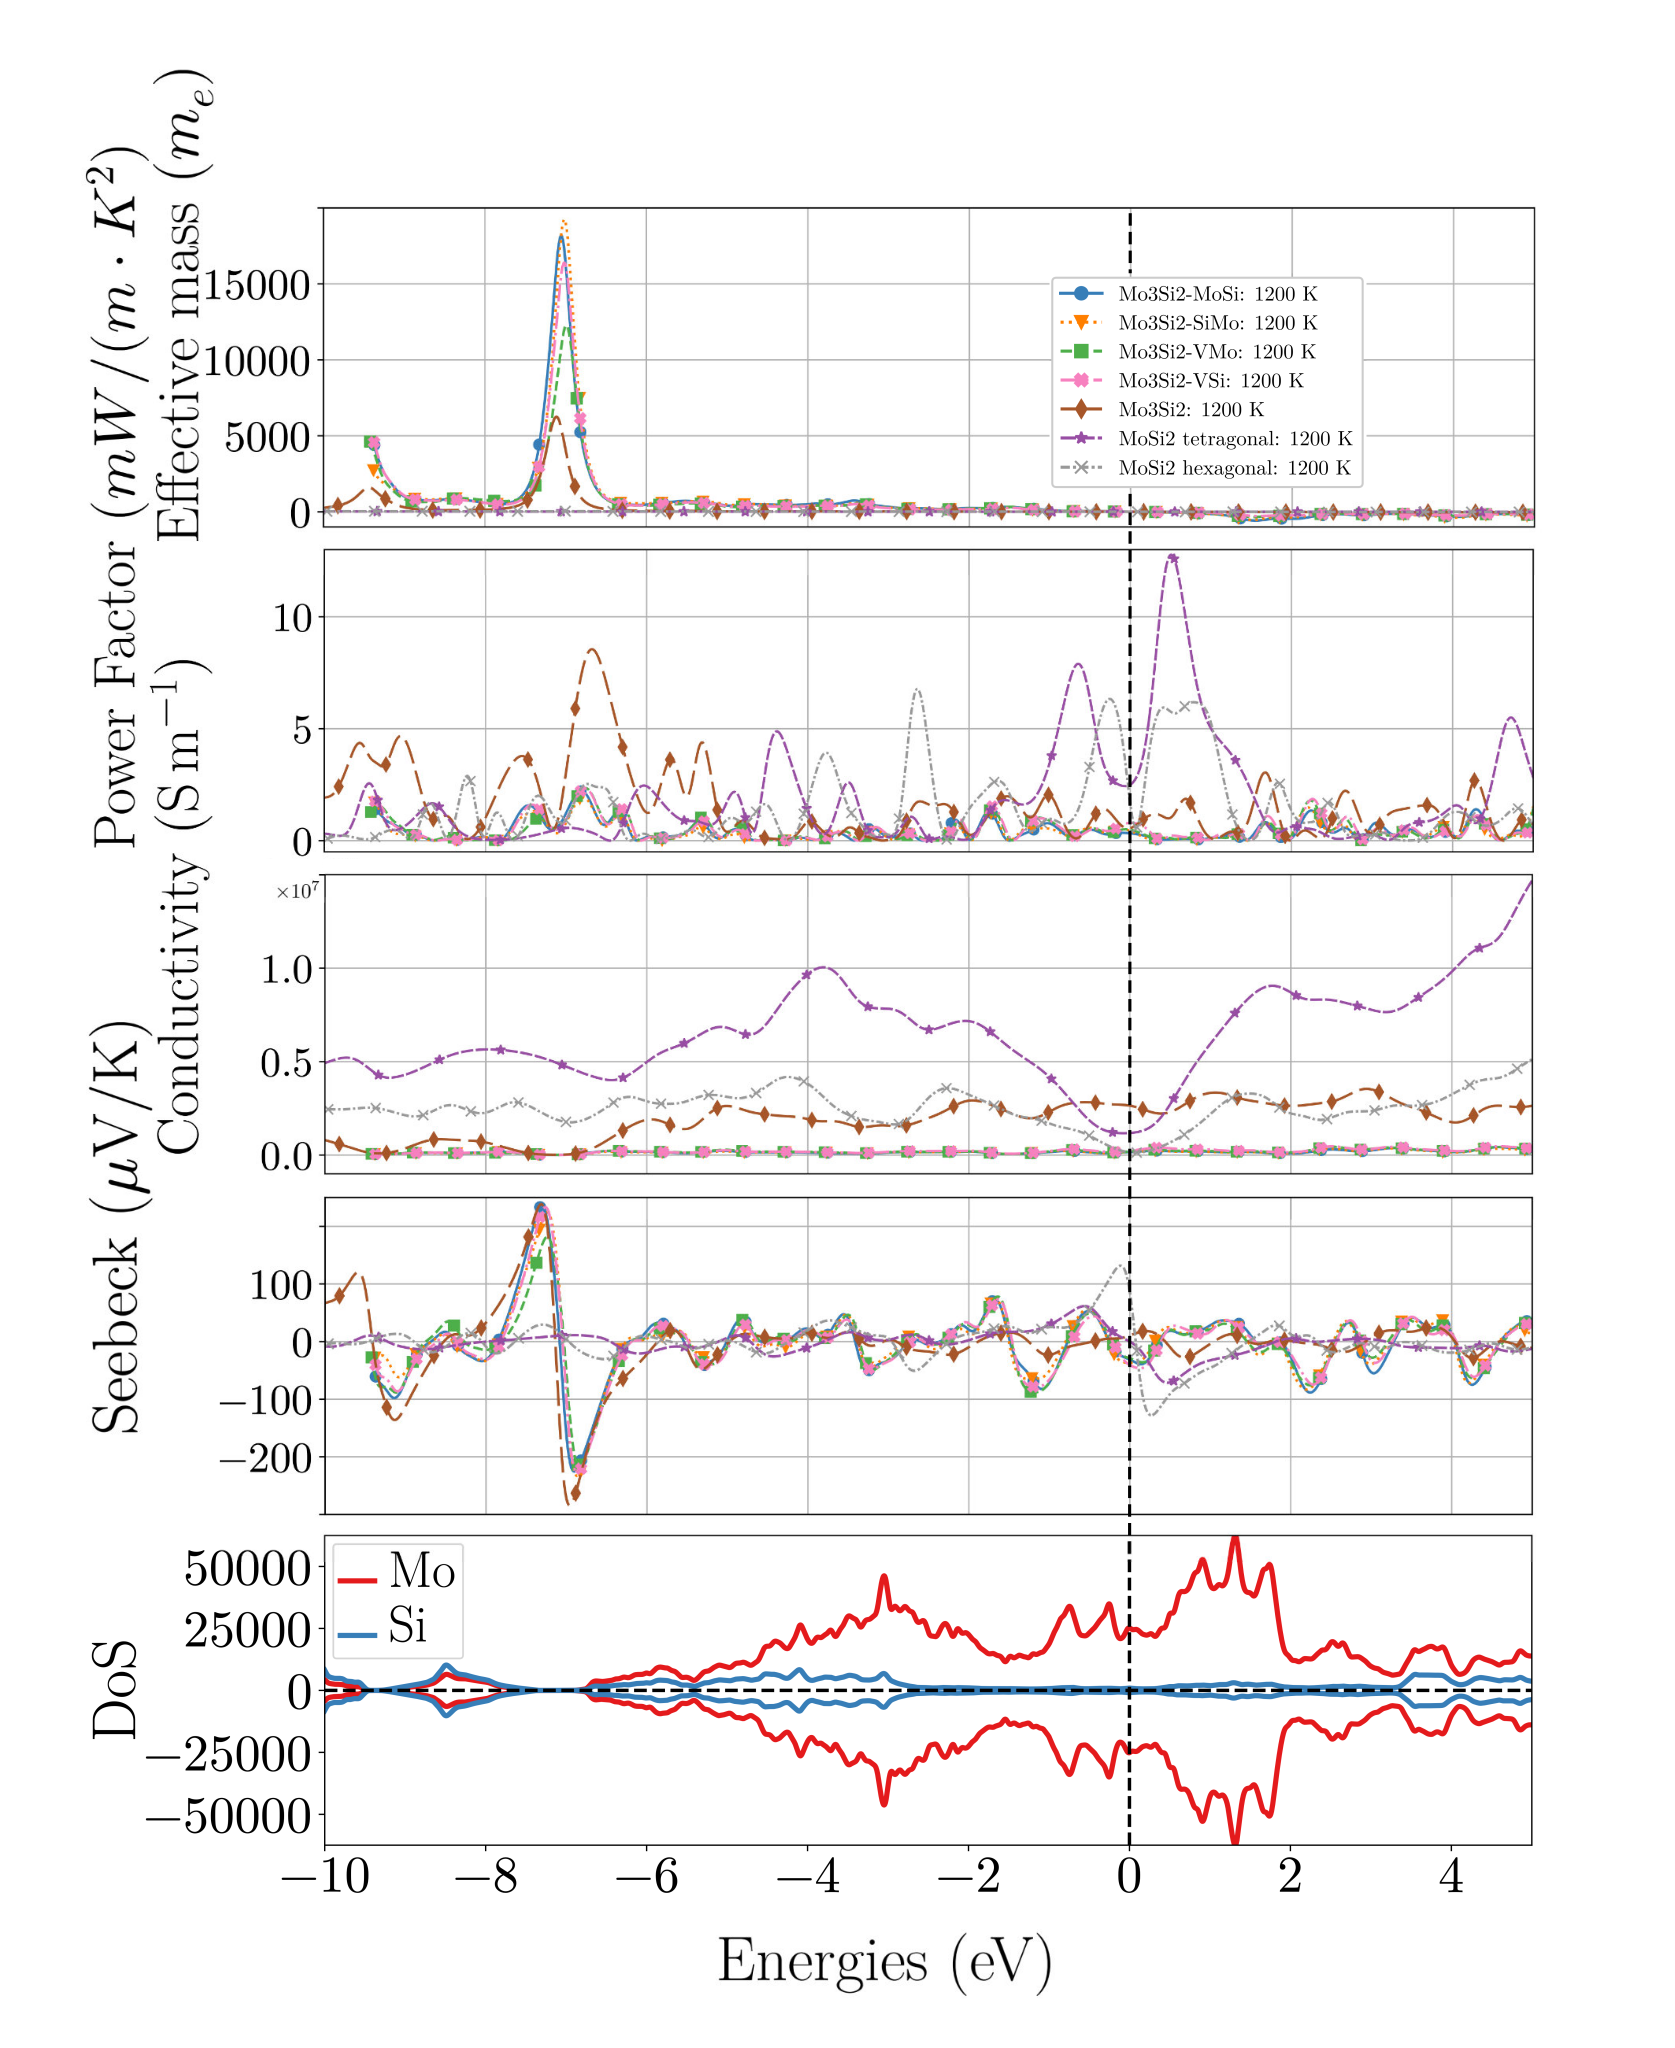
\includegraphics[width=1.08\textwidth]{E-plots}
\caption{Caption provided on the next page.}
\end{figure}
\addtocounter{figure}{-1}
\begin{figure} [t!]
  \caption{The density of states of silicon and molybdenum is plotted alongside four other quantities on a shared energy axis, where the zero energy is the Fermi energy. The quantities, in order from bottom to top, are the Seebeck coefficient, the conductivity, the power factor and the effective mass. All four quantities each regard the pristine $\text{Mo}\text{Si}_2$ structures (tetragonal and hexagonal); the $\text{Mo}_3\text{Si}_2$ pristine structure, and the four $\text{Mo}_3\text{Si}_2$ defect-containing structures. The density of states plot is that of $\text{Mo}_3\text{Si}_2$ pristine. Those of $\text{Mo}\text{Si}_2$ are two orders of magnitude larger in value, and are omitted for that reason.}
\end{figure}

\clearpage

\subsection{Material structure}

The pristine Mo3Si2 compound has roughly as many Mo-Si bonds as the hexagonal, pristine MoSi2 compound, as can be seen in table \ref{tab:mo-bonds}.
Pristine Mo3Si2, however, has a smaller average bond length than the MoSo2 compounds.
The Si vacancy Mo3Si2 compound notably has two bonds less than the Mo vacancy compound \ref{tab:mo-bonds}.
The minimal bond length rises significantly for the Si vacancy compared to the other Mo3Si2 defects; as does the maximal bond length for the MoSi defect.

% TODO compare with experiment
\begin{table}[t!]
  \small
  \centering
  \caption{The number of Mo-Si bonds and their minimum, maximum and average bond length (BL).}
\begin{tabular}{@{}lllll@{}}
\toprule
\text {Compound} & \text{Num. bonds} & \text{Min BL (\angstrom)} & \text{Max BL (\angstrom)} & \text{Avg BL (\angstrom)} \\
\midrule
\text{Mo}_3\text{Si}_2\text{ prist.} & 20 & 2.527149447674506 & 2.583837169568993 & 2.565183303531114 \\
\text{Mo}_3\text{Si}_2\text{-MoSi} & 507 & 2.4713831013822998 & 3.0203054431172864 & 2.561940116145447 \\
\text{Mo}_3\text{Si}_2\text{-SiMo} & 511 & 2.4603724721476348 & 2.830573726108845 & 2.5635721997455305 \\
\text{Mo}_3\text{Si}_2\text{-VMo} & 506 & 2.490718341670391 & 2.7230431789162726 & 2.563755719419874 \\
\text{Mo}_3\text{Si}_2\text{-VSi} & 504 & 2.563755719419874 & 2.631947428081024 & 2.5622698386685836 \\
\text{Mo}\text{Si}_2\text{ prist. tetr.} & 2 & 2.6198256693192206 & 2.6198256693192206 & 2.6198256693192206 \\
\text{Mo}\text{Si}_2\text{ prist. hexa.} & 18 & 2.5805119710876046 & 2.6535845258140287 & 2.6048716472411018
\end{tabular}
  \label{tab:mo-bonds}
\end{table}

\begin{figure}[b!]
\label{fig:mat-pristine}
\centering
\includegraphics[width=0.75\textwidth]{img/Mo3Si2-pristine}
\caption{The $\text{Mo}_3\text{Si}_2$ pristine structure (spacegroup P4/mbm number 127), on the left pictured with the $c$ axis pointed towards the screen, and on the right in the standard orientation.}
\end{figure}

\begin{figure}
\label{fig:mo3si2-defects-b}
\centering
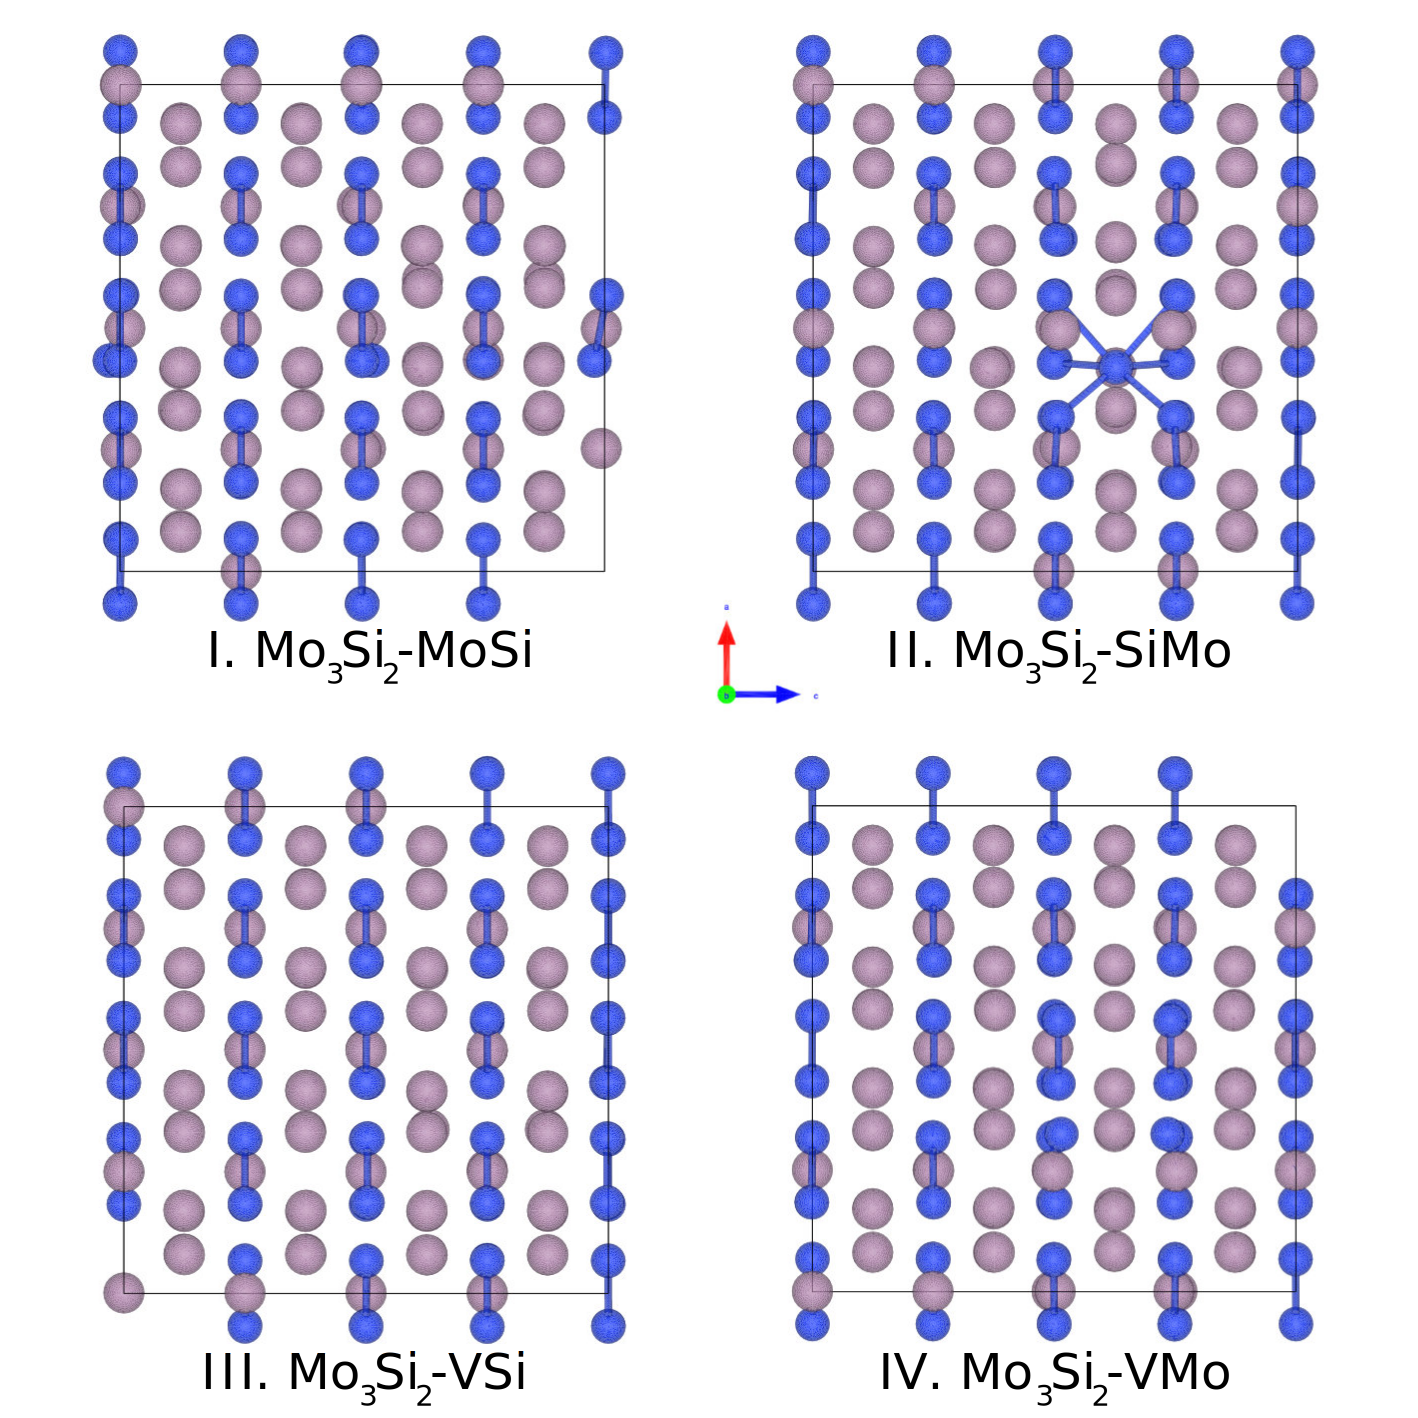
\includegraphics[width=0.6\textwidth]{img/Mo3Si2-defects-b}
\caption{The four defect variants of $\text{Mo}_3\text{Si}_2$ we investigated, all plotted with the $b$ axis facing the camera and the $a$ axis pointing upwards. On the top left corner, the $\text{Mo}_{Si}$ defect (spacegroup Amm2 number 38), which gives rise to a tilted substructure with respect to the pristine lattice, to be seen on the rightmost edge. On the top right corner, the $\text{Si}_{Mo}$ defect (spacegroup Amm2 number 38), with more strongly bonded atoms than the pristine. On the bottom left corner, the silicon vacancy defect (spacegroup Amm2 number 38); and on the bottom right, the molybdenum vacancy defect (spacegroup Amm2 number 38).}
\end{figure}

\clearpage

\subsection{Band structure}

\begin{figure}[b!]
\centering
\begin{subfigure}{.5\textwidth}
  \centering
\includegraphics[width=\linewidth]{img/partial_dos_MoSi2_tetragonal.pdf}
  \caption{}
\label{fig:DOS-mosi2-hexagonal}
\end{subfigure}%
\begin{subfigure}{.46\textwidth}
  \centering
\includegraphics[width=\linewidth]{img/partial_dos_MoSi2_hexagonal.pdf}
  \caption{}
\label{fig:DOS-mosi2-tetragonal}
\end{subfigure}
\caption{This figure displays the partial density of states of the pristine tetragonal $\text{Mo}\text{Si}_2$ structure. On the y-axis the density of states is shown; on the x-axis the energy of the electrons relative to the Fermi-energy is shown. --OTHER FIGURE--. This figure displays the partial density of states of the pristine hexagonal $\text{Mo}\text{Si}_2$ structure. On the y-axis the density of states is shown; on the x-axis the energy of the electrons relative to the Fermi-energy is shown.}
\end{figure}


As seen in figure \ref{fig:DOS-mosi2-tetragonal} and the bottom-most graph of \ref{fig:e-plots}, the tetragonal $\text{Mo}\text{Si}_2$ structure does not have a complete band gap; whereas the hexagonal structure does. $\text{Mo}_3\text{Si}_2$ has metal-like properties as a result of the lack of band gap at the Fermi energy. 
The presence of the band gap is reflected in the conductivity of electrons near the Fermi energy, as shown figure \ref{fig:e-plots}, where it can be seen that bands near the Fermi energy have a lower conductivity for materials with a band gap or partial band gap. 
Notably, the defective structures conduct poorly overall, which may be attributed to the defect concentration of these structures not being representative of defect concentrations of actual semiconductors. 
% TODO rewrite
The defective structures consisted of 160 atoms, one of which being the point defect itself, resulting in a defect concentration of approximately $10^{-2}$ mol defects per mol. 
As is shown in figure \ref{fig:defect-form-temp} defects at this concentration do not occur at reasonable temperatures.

The effective mass of electrons, $m^*=\hbar^2\left(d^2 E(k) / d k^2\right)^{-1}$, is inversely proportional to the curvature of the bands. In fig \ref{fig:e-plots} a sharp peak can be seen near -7 and -10 eV for the pristine $\text{Mo}_3\text{Si}_2$ and the defective $\text{Mo}_3\text{Si}_2$ structures. 
This can be explained by the band gaps for $\text{Mo}_3\text{Si}_2$ at these energy levels, where bands are flattened and curved, thus causing a high effective mass. 
The pristine $\text{Mo}_3\text{Si}_2$ structure peaks significantly lower than the other materials. Given that a low effective mass is desirable \cite{alma9939162912205131}, this suggests that the pristine structure performs better than the defective structures.

\begin{figure}
\label{fig:bs-mo3si2}
\centering
\includegraphics[width=0.75\textwidth]{img/bs_Mo3Si2}
\caption{This figure shows the band structure of Mo\textsubscript{3}Si\textsubscript{2} across high symmetry points.}
\end{figure}


\begin{figure}
\centering
\begin{subfigure}{.5\textwidth}
  \centering
  \includegraphics[width=\linewidth]{bs_MoSi2_tetragonal}
  \caption{}
\label{fig:bs-mosi2-tetra}
\end{subfigure}%
\begin{subfigure}{.5\textwidth}
  \centering
  \includegraphics[width=\linewidth]{bs_MoSi2_hexagonal}
  \caption{}
\label{fig:bs-mosi2-hexa}
\end{subfigure}
\caption{Pictured on the left is the band structure of the pristine tetragonal MoSi\textsubscript{2} structure across high symmetry points; on the right, the band structure of the pristine hexagonal MoSi\textsubscript{2} structure.}
\label{fig:bs_MoSi2}
\end{figure}

\clearpage

\subsection{Defect concentration}

The intrinsic defect concentrations determine the carrier concentrations in undoped systems. These concentrations are directly dependent on the formation energy, which is calculated according to \ref{eq:formationenergy}, and so on the binding energies of the atoms and the energy of the defective and pristine system \ref{eq:defectconcentration}. The carrier concentration will ultimately affect both the Seebeck coefficient and the resistivity.

% TODO tetragonal? Pristine? Hexagonal?
\begin{table}[t!]
\caption{The defect formation energies of both MoSi\textsubscript{2} and Mo\textsubscript{3}Si\textsubscript{2} in eV.}
\centering
\begin{tabular}{@{}lllll@{}}
\toprule
      & V\textsubscript{Si}  & V\textsubscript{Mo}  & Mo\textsubscript{Si} & Si\textsubscript{Mo} \\ \midrule
MoSi\textsubscript{2} & 11.6 & 24.7 & 2.9  & 4.8  \\
Mo\textsubscript{3}Si\textsubscript{2} & 12.5 & 22.7 & 2.0  & 1.4 
\end{tabular}
\end{table}


\begin{figure}[b!]
\centering
\begin{subfigure}{.5\textwidth}
  \centering
  \includegraphics[width=\linewidth]{img/mosi2defects.pdf}
  \caption{}
  \label{fig:sub1}
\end{subfigure}%
\begin{subfigure}{.5\textwidth}
  \centering
  \includegraphics[width=\linewidth]{img/mo3si2defects.pdf}
  \caption{}
  \label{fig:sub2}
\end{subfigure}
\caption{The defect concentration as a function of temperature is shown for MoSi\textsubscript{2} on the left, and Mo\textsubscript{3}Si\textsubscript{2} on the right.}
\label{fig:defect-form-temp}
\end{figure}



As seen in figure \ref{fig:defect-form-temp} silicon vacancies are much more prevalent than molybdenum vacancies as they have a lower defect formation energy for both $\text{Mo}\text{Si}_2$ and $\text{Mo}_3\text{Si}_2$, but in the case of antisites for $\text{Mo}_3\text{Si}_2$ the $\text{Si}_{Mo}$ antisite is more prevalent than the $\text{Mo}_{\text{Si}}$ antisite, whereas for $\text{Mo}\text{Si}_2$ it is the other way around. 

\subsection{Seebeck coefficient}


\begin{figure}[t!]
\centering
\begin{subfigure}{.5\textwidth}
  \centering
  \includegraphics[width=\linewidth]{allmats_S_temp_doping_n}
  \caption{}
  \label{fig:sub1}
\end{subfigure}%
\begin{subfigure}{.5\textwidth}
  \centering
  \includegraphics[width=\linewidth]{allmats_S_temp_doping_p}
  \caption{}
  \label{fig:sub2}
\end{subfigure}
\caption{The Seebeck coefficient as a function of temperature at a set carrier concentration. On the left the Seebeck coefficient is shown for n-type structures, and on the right for p-type structures.}
\label{fig:S-Temp}
\end{figure}


The Seebeck coefficient seems to be strongly affected by the carrier concentration in the structures, changing sign at a certain concentration for the hexagonal $\text{Mo}\text{Si}_2$ structure in case of an n-type TE, as seen in figure \ref{fig:S-Doping}. This may be attributed to the band gap in the material. 
interestingly, the Seebeck coefficient of the metallic $\text{Mo}_{3}\text{Si}_{2}$ also changes sign at high carrier concentrations. This should not happen in a metal, it is likely that the simulations break down for Carrier concentrations around ~$10^{22}$. moreover, all of the defective $\text{Mo}_{3}\text{Si}_{2}$ have a sign opposite to that of the pristine structure.

In figure \ref{fig:S-Temp} the relation between the Seebeck coefficient and temperature is shown. For all structures the absolute value of the Seebeck coefficient increases with temperature up until about 1400 K. 


\begin{figure}[b!]
\centering
\begin{subfigure}{.5\textwidth}
  \centering
  \includegraphics[width=\linewidth]{allmats_S_doping_temp_n}
  \caption{}
  \label{fig:sub1}
\end{subfigure}%
\begin{subfigure}{.5\textwidth}
  \centering
  \includegraphics[width=\linewidth]{allmats_S_doping_temp_p}
  \caption{}
  \label{fig:sub2}
\end{subfigure}
\caption{The Seebeck coefficient as a function of the carrier concentration. On the left the Seebeck coefficient is shown for n-type structures, and on the right for p-type structures.}
\label{fig:S-Doping}
\end{figure}

\subsection{Conductivity}

\begin{figure}[t!]
\centering
\begin{subfigure}{.5\textwidth}
  \centering
  \includegraphics[width=\linewidth]{allmats_C_temp_doping_n}
  \caption{}
  \label{fig:sub1}
\end{subfigure}%
\begin{subfigure}{.5\textwidth}
  \centering
  \includegraphics[width=\linewidth]{allmats_C_temp_doping_p}
  \caption{}
  \label{fig:sub2}
\end{subfigure}
\caption{Conductivity of the structures as a function of temperature at a set carrier concentration. On the left the conductivity is shown for n-type structures, and on the right for p-type structures.}
\label{fig:C-Temp}
\end{figure}

The electric conductivity does not strongly depend on temperature, especially for the defective systems. This result does not correspond to the temperature dependence of conductivity of real materials. This may be attributed to the omittance of phonon interactions in BoltzTrap2, which dominate conductivity above [look up what temps] K. The defects negatively impact the conductivity for all defects, as expected from perturbations in the lattice. Also, the pristine $\text{Mo}_3\text{Si}_2$ structure has a much higher conductivity than both $\text{Mo}\text{Si}_2$ phases. 



\begin{figure}[b!]
\centering
\begin{subfigure}{.5\textwidth}
  \centering
  \includegraphics[width=\linewidth]{allmats_C_doping_temp_n}
  \caption{}
  \label{fig:sub1}
\end{subfigure}%
\begin{subfigure}{.5\textwidth}
  \centering
  \includegraphics[width=\linewidth]{allmats_C_doping_temp_p}
  \caption{}
  \label{fig:sub2}
\end{subfigure}
\caption{The conductivity of all materials as a function of the carrier concentration. On the left the conductivity is shown for n-type structures, and on the right for p-type structures}
\label{fig:C-Doping}
\end{figure}


In fig [] it can be seen that $\text{Mo}_3\text{Si}_2$ is not significantly affected by the carrier concentration. This may be because of the lack of a band gap near the Fermi energy. 
% [band gap visible from increase in conductivity near 10^21]
% [compare conductivity with formulas from slides]
% [carrier conc. physical at 10^23]

\subsection{The Seebeck Coefficient}

\begin{table}[t!]
  \small
  \centering
  \caption{Largest predicted Seebeck coefficient, evaluated at a carrier concentration of TODO, for each compound, additionally related to the spacegroup. }
\begin{tabular}{@{}lllll@{}}
\toprule
\text {Compound} & \text{Spacegroup} & \text{$|S_{\text{max}}|$ ($\mu$V/K)} & \text{$T$ (K)} & \text{Doping} \\
\midrule
\text{Mo}_3\text{Si}_2\text{ prist.} & \text{P4/mbm (number 127)} & 15 & 1800 & \text{n}  \\
\text{Mo}_3\text{Si}_2\text{-MoSi} & \text{Amm2 (number 38)} & 35 & 1200 & \text{n}  \\
\text{Mo}_3\text{Si}_2\text{-SiMo} & \text{Amm2 (number 38)} & 38 & 1200 & \text{n}  \\
\text{Mo}_3\text{Si}_2\text{-VMo} & \text{Amm2 (number 38)} & 30 & 1200 & \text{n}  \\
\text{Mo}_3\text{Si}_2\text{-VSi} & \text{Amm2 (number 38)} & 44 & 1200 & \text{n}  \\
\text{Mo}\text{Si}_2\text{ prist. tetr.} & \text{I4/mmm (number 139)} & 28 & 1800 & \text{n}  \\
\text{Mo}\text{Si}_2\text{ prist. hexa.} & \text{P6-222 (number 180)} & 125 & 900 & \text{n}
\end{tabular}
  \label{tab:seebeck}
\end{table}

In table \ref{tab:seebeck} we display the largest predicted Seebeck coefficients amongst varying temperature and doping type.
We additionally include the compound's spacegroup, as it is apparent from \ref{tab:seebeck} that there is a relationship between it and the Seebeck coefficient.


\subsection{Power Factor}

\begin{figure}[b!]
\centering
\begin{subfigure}{.5\textwidth}
  \centering
  \includegraphics[width=\linewidth]{allmats_Po_temp_doping_n}
  \caption{}
  \label{fig:sub1}
\end{subfigure}%
\begin{subfigure}{.5\textwidth}
  \centering
  \includegraphics[width=\linewidth]{allmats_Po_temp_doping_p}
  \caption{}
  \label{fig:sub2}
\end{subfigure}
\caption{The power factor of the structures plotted as a function of temperature. On the left the power factor is shown for n-type structures, and on the right for p-type structures.}
\label{fig:Po-T}
\end{figure}

The power factor shows a strong dependency on temperature, increasing the power factor as the temperature rises. This may, however, not reflect the power factor in experimental data, because the varying relaxation time is not taken into account in BoltzTrap2. 
Also, the graph may not represent the actual scaling of the power factor because the carrier concentration is chosen arbitrarily. 
The tetragonal $\text{Mo}\text{Si}_{2}$ structure seems to have the most favourable power factor at this carrier concentration. The competing structure, hexagonal $\text{MoSi}_{2}$, can be tuned to have a Seebeck coefficient that is almost twice as high as that of the tetragonal $\text{Mo}\text{Si}_{2}$ structure at a carrier concentration of around $10^{21}$ $\text{cm}^{-3}$. Additionally in this range, the conductivity in these materials is much higher. The increase of both parameters would positively affect the power factors for these materials. It is evident from the figures \ref{fig:S-Doping} and \ref{fig:C-Doping} that these two materials would serve better as n-type semiconductors than p-type semiconductors.

\begin{figure}[b!]
\centering
\begin{subfigure}{.5\textwidth}
  \centering
  \includegraphics[width=\linewidth]{allmats_Po_doping_temp_n}
  \caption{}
  \label{fig:sub1}
\end{subfigure}%
\begin{subfigure}{.5\textwidth}
  \centering
  \includegraphics[width=\linewidth]{allmats_Po_doping_temp_p}
  \caption{}
  \label{fig:sub2}
\end{subfigure}
\caption{The power factor of the structures plotted as a function of the carrier concentration. On the left the power factor is shown for n-type structures, and on the right for p-type structures.}
\label{fig:Po-doping}
\end{figure}

\clearpage

\section{Conclusion}

In this paper we studied the power factor of two molybdenum silicides, $\text{Mo}_3\text{Si}_2$ and $\text{MoSi}_2$, at high temperatures. The power factor is a factor in the figure of merit, is determined by the Seebeck coefficient, electrical conductivity and temperature. The study used computational analysis of previous research data on the band energies of the materials, obtained through density functional theory. The transport properties and Seebeck coefficient were varied as a function of carrier density, temperature, and chemical potential, and the data was compared to find the most favourable structure for thermoelectric material, both for p-type as well as n-type materials. The stability of each of the defects, such as antisites and vacancies, was determined by calculating the equilibrium defect concentration.  
For both n-type and p-type materials, the power factor was the highest for the tetragonal $\text{MoSi}_{2}$ structure at a carrier concentration of around $10^22$ $\text{cm}^{-3}$ as displayed in figure \ref{fig:Po-doping}. The power factor is, however, sensitive to temperature as seen in figure \ref{fig:Po-T}, even when phonon scattering was not accounted for. This shows that the choice of material should depend on the eventual operating temperature of thermoelectric device. This temperature dependence is mainly attributed to the temperature dependence of the Seebeck coefficient. Figure \ref{fig:Po-T} also shows that at low temperatures point defects may increase the power factor of the thermoelectric material. 
[defect concentrations]



\section{Future studies}

[short mention of gw?]
[test defect concentrations that reflect concentration at application temperature, as these defects concentrations are probably way above what is expected from realistic concentrations]
[study that takes phonon contributions into account]

A research group at the Advanced Research Center for Nanolithography (ARCNL) has demonstrated a method that could potentially be used for characterising the defects in the volume of a thermoelectric material [128]. The group used coherent extreme-ultraviolet pulses from high-harmonic generation to produce a spectrogram on which the different point defects manifest as unique visual signatures. This technique is best suited for materials with a band-gap, thus semiconductors. The results are promising and garner further attention as it is rare to find effective methods for characterising point defects in the bulk of thermoelectrics.

TODO replace with another group, this has to be a technique.
A different group at ARCNL demonstrated an essential dependency on a $\text{Mo}_{x}\text{Si}_{y}$ material [28]. The group produces a laser pulse in the extreme ultraviolet, for which it is hard to find a mirror that does not absorb it. A thin layer of a molybdenum silicide compound has been found to be highly effective in this application, and is currently in use in the field. The exact mechanism of this reflectivity is not well understood. A better understanding of the behaviour of molybdenum silicides will undoubtedly lead to essential knowledge for the field of high-energy laser mirrors.



\section{Author contribution statement}
All authors contributed to advancing the methodology of this paper. Marshall was in charge of processing and visualizing DFT data. Broerse and Marshall were the main authors of this paper. 


\medskip

\cleardoublepage

\printbibliography

\cleardoublepage

\pagebreak

\section{Appendix A - Supplementary Material Structure Information}

\begin{figure}
\label{fig:mo3si2-defects-a}
\centering
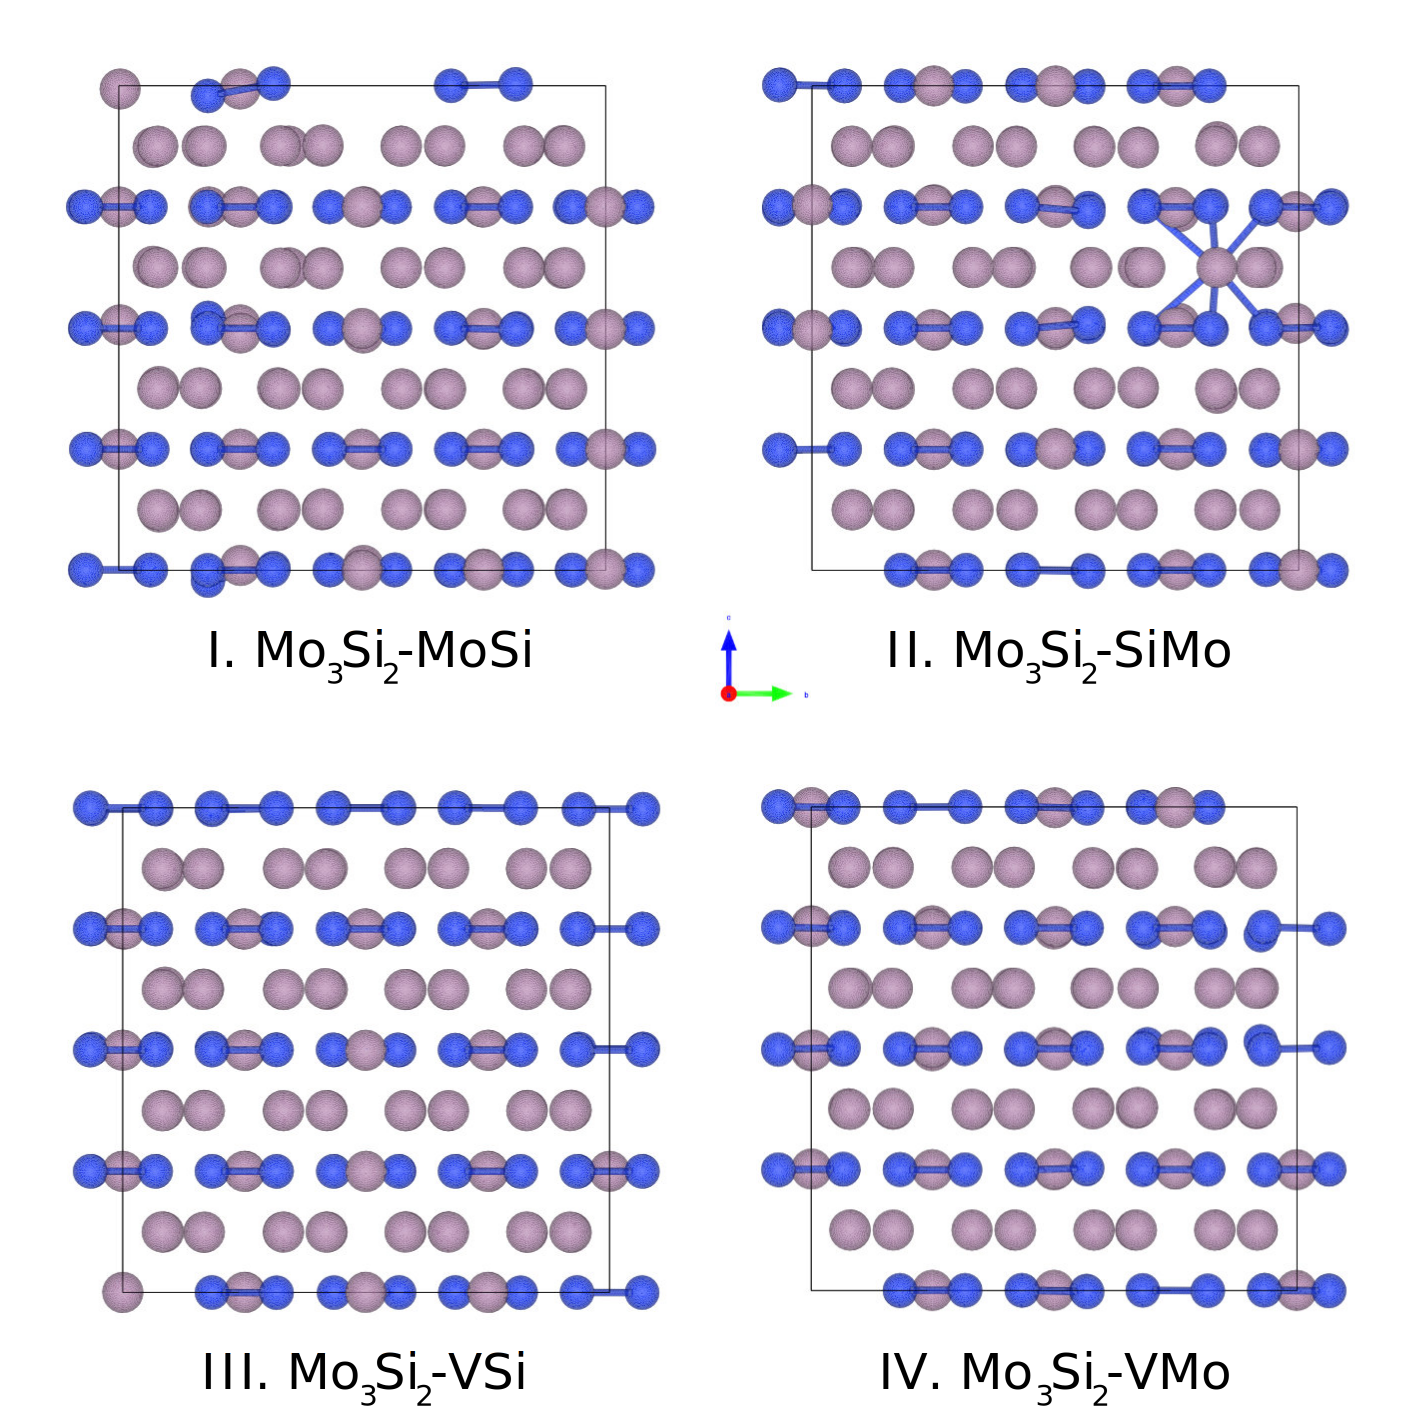
\includegraphics[width=0.6\textwidth]{img/Mo3Si2-defects-a}
\caption{The four defect variants of $\text{Mo}_3\text{Si}_2$ we investigated, all plotted with the $a$ axis facing the camera and the $c$ axis pointing upwards. On the top left corner, the $\text{Mo}_{Si}$ defect (spacegroup Amm2 number 38), which gives rise to a tilted substructure with respect to the pristine lattice, to be seen on the top-most edge. On the top right corner, the $\text{Si}_{Mo}$ defect (spacegroup Amm2 number 38), with more strongly bonded atoms than the pristine. On the bottom left corner, the silicon vacancy defect (spacegroup Amm2 number 38); and on the bottom right, the molybdenum vacancy defect (spacegroup Amm2 number 38).}
\end{figure}

\begin{figure}
\label{fig:mo3si2-defects-c}
\centering
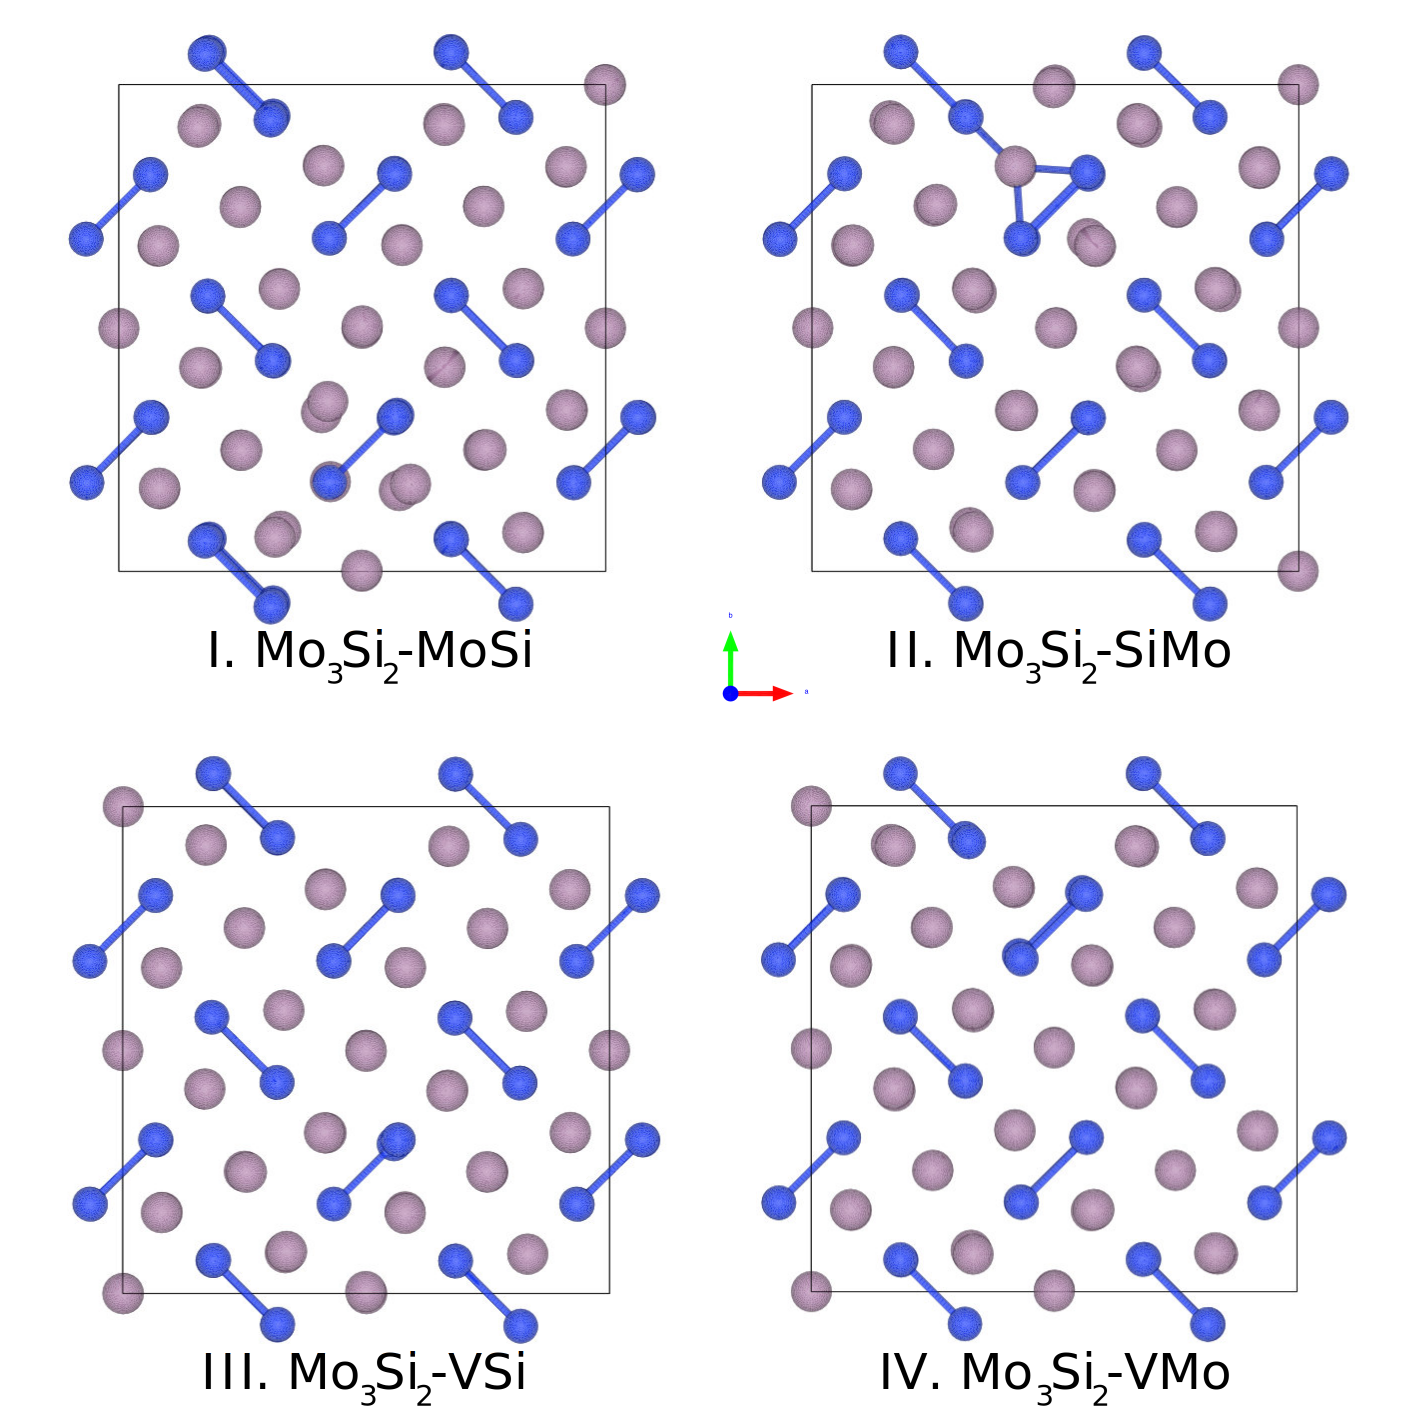
\includegraphics[width=0.6\textwidth]{img/Mo3Si2-defects-c}
\caption{The four defect variants of $\text{Mo}_3\text{Si}_2$ we investigated, all plotted with the $c$ axis facing the camera and the $b$ axis pointing upwards. On the top left corner, the $\text{Mo}_{Si}$ defect (spacegroup Amm2 number 38). On the top right corner, the $\text{Si}_{Mo}$ defect (spacegroup Amm2 number 38), with more strongly bonded atoms than the pristine. On the bottom left corner, the silicon vacancy defect (spacegroup Amm2 number 38); and on the bottom right, the molybdenum vacancy defect (spacegroup Amm2 number 38).}
\end{figure}

% \section{Appendix B}

% \subsection{Mo3Si2-MoSi}

% \subsubsection{Reciprocal cell vectors (1/\angstrom)}

% \begin{equation}
% \begin{array}{cccc}
% \text { b } & x & y & z \\
% b_1 & 0.9484463952 & 0.0000000000 & 0.0000000000 \\
% b_2 & 0.0000000000 & 0.9484463952 & 0.0000000000 \\
% b_3 & 0.0000000000 & 0.0000000000 & 1.9066222087
% \end{array}
% \end{equation}

% \subsubsection{High-symmetry points (scaled units)}

% \begin{equation}
% \begin{array}{cccc}
% \text { Label } & k_1 & k_2 & k_3 \\
% A & 0.5 & 0.5 & 0.5 \\
% \Gamma & 0.0 & 0.0 & 0.0 \\
% M & 0.5 & 0.5 & 0.0 \\
% R & 0.0 & 0.5 & 0.5 \\
% X & 0.0 & 0.5 & 0.0 \\
% Z & 0.0 & 0.0 & 0.5
% \end{array}
% \end{equation}

% \section{Appendix C}

% \begin{equation}
% \begin{array}{llll}
% \text {Lattice} & \text{Bravais lat. type} & \text{Ext. Bravais lat. symbol} & \text{Spacegroup} \\
% \text{Mo}_3\text{Si}_2\text{ pristine} & \text{tP} & \text{tP1 (with i.s.)} & \text{P4/mbm (n. 127)}  \\
% \text{Mo}_3\text{Si}_2\text{-MoSi} & \text{oA} & \text{oA1 (no i.s.)} & \text{Amm2 (number 38)}  \\
% MoSi2, pristine, tetragonal & 0.9484463952 & 0.0000000000 & 0.0000000000  
% \end{array}
% \end{equation}

% \section{Appendix D}


\end{document}

% TODO:
% - link findings to existing studies: compare to power factors of existing materials
% - figures in correct places, do this at last
% - compare binding energy to bond lengths
% - bond angles?
% - mention that the results are not optimized, 2dimensionally
% - repeat seebeck table for power factor
% - verify values of tables, as they are taken by eye from the plots
% - verify no faults in bibliography

